
\subsection{Two dimensional uniform dataset}

\begin{figure}
  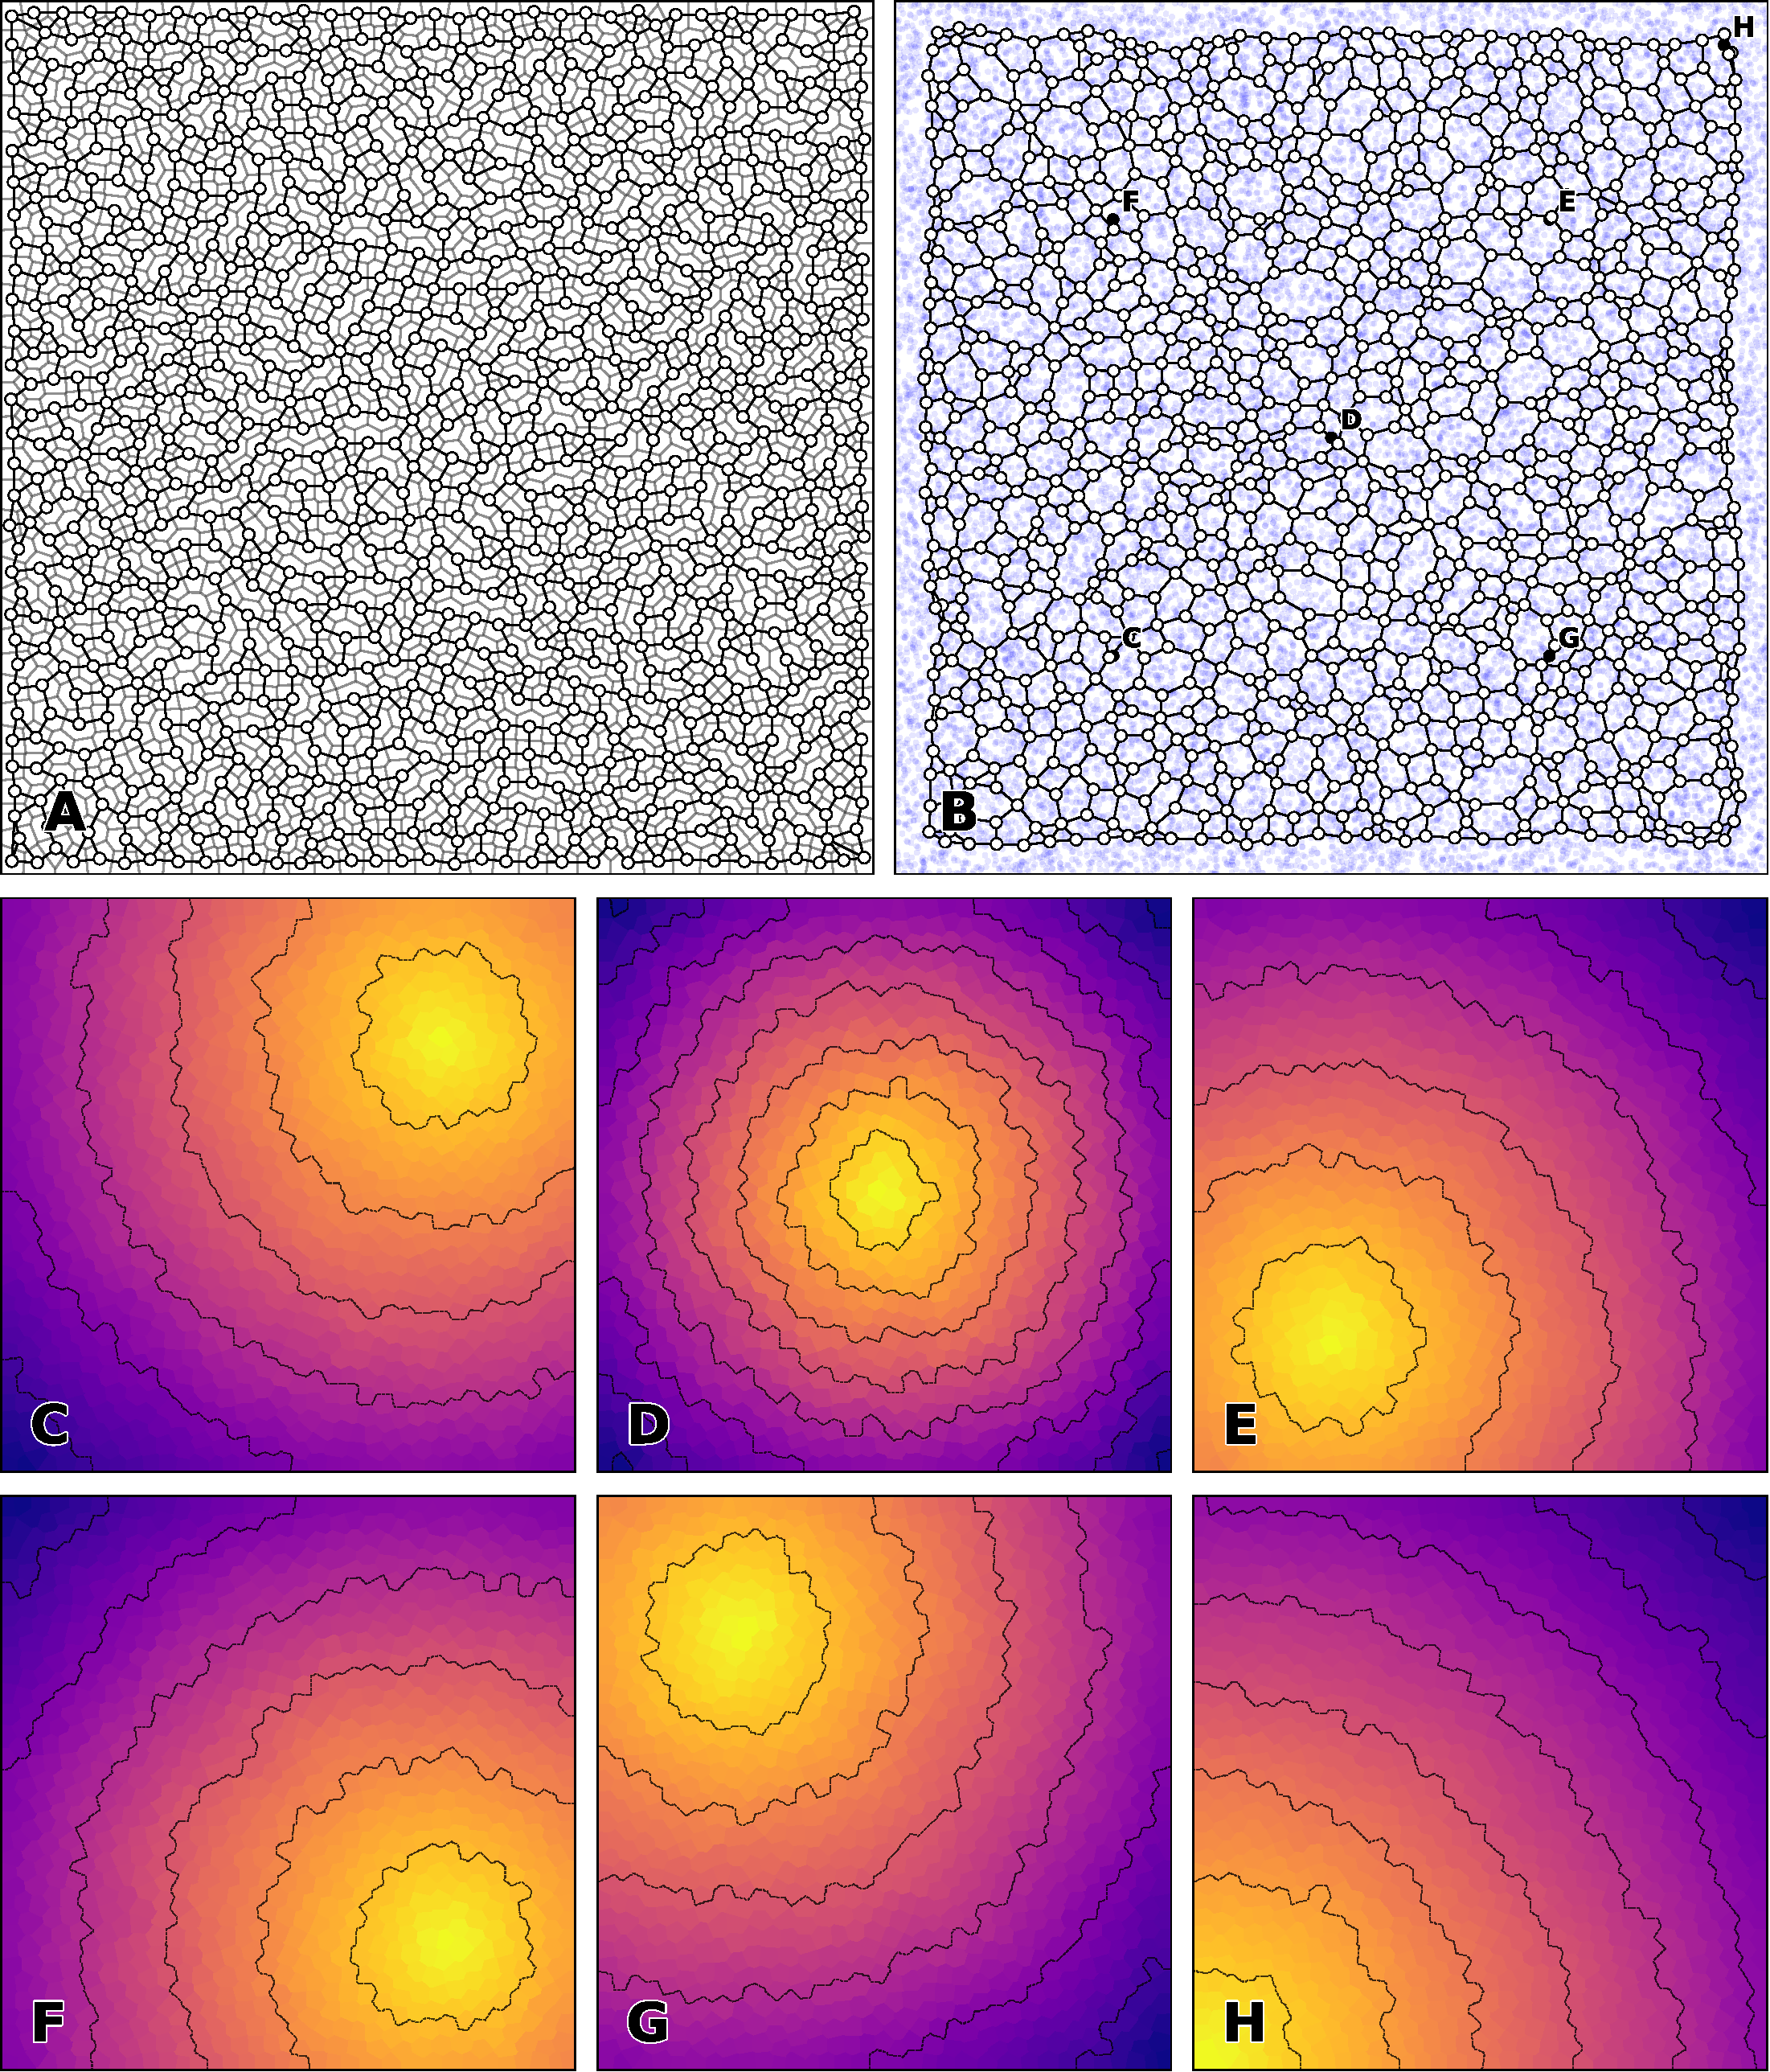
\includegraphics[width=\columnwidth]{experiment-2D-uniform.pdf}
  \vspace{2mm}
  \centering
  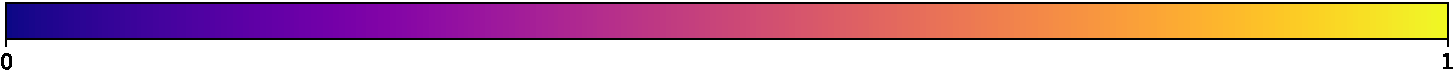
\includegraphics[width=.975\columnwidth]{colormap.pdf}
  %
  \caption{%
  %
  {\bfseries \sffamily Two dimensional uniform dataset (results)}
  %
  Randomized SOM made of $1024$ neurons with a $2$-nearest neighbors induced topology. Model has been trained for $25,000$ epochs on two-dimensional points drawn from a uniform distribution on the unit square. \textbf{A} Map topology in neural space. \textbf{B} Map topology in data space. \textbf{C to H} Receptive field of the map for six samples.
  %
  }
  \label{fig:2D-uniform:results}
\end{figure}
